\documentclass[conference,a4paper]{IEEEtran}
\IEEEoverridecommandlockouts
\usepackage[spanish,es-noshorthands,es-tabla,es-nodecimaldot]{babel}
\usepackage{amsmath,amssymb}
\usepackage{fontspec}
\setmainfont{texgyretermes}[Extension=.otf, UprightFont=*-regular, BoldFont=*-bold, ItalicFont=*-italic, BoldItalicFont=*-bolditalic]
\setmonofont{texgyrecursor}[Extension=.otf, UprightFont=*-regular, BoldFont=*-bold, ItalicFont=*-italic, BoldItalicFont=*-bolditalic, Scale=0.95]
\usepackage{graphicx}
\usepackage{booktabs}
\usepackage{array}
\usepackage{cite}
\usepackage{url}
\usepackage[hidelinks]{hyperref}
\hypersetup{pdftitle={Evaluación de la calidad de un dashboard de vigilancia de malaria con ISO/IEC 25010},
  pdfauthor={J. M. Cari Quispe, D. W. Chura Monroy, O. F. Lopez Arela, A. J. Phocco Tapia, M. E. Zegarra Puma},
  pdfsubject={Calidad de Software, Trabajo Parcial 6, UNSA 2026-B},
  pdfkeywords={ISO/IEC 25010, ISO/IEC 25040, GQM, malaria, tablero de control},
  pdfcreator={Equipo TP6 - Calidad de Software UNSA}}
\def\UrlBreaks{\do\/\do-\do.\do_}
\newcolumntype{L}[1]{>{\raggedright\arraybackslash}p{#1}}
\graphicspath{{figuras/}}

\begin{document}

\title{Evaluación de la calidad de un dashboard de vigilancia de malaria con ISO/IEC~25010: métricas GQM automatizadas, clasificación de fallos por origen y tablero de control}

\author{
\IEEEauthorblockN{Juan Manuel Cari Quispe, Daniel Wilston Chura Monroy, Ower Frank Lopez Arela,\\ Alejandro Josue Phocco Tapia y Mauricio Eduardo Zegarra Puma}
\IEEEauthorblockA{Escuela Profesional de Ingeniería de Sistemas, Universidad Nacional de San Agustín de Arequipa\\
Arequipa, Perú · Curso Calidad de Software, Trabajo Parcial 6 · octubre de 2026\\
Producto: \url{https://vigisalud-malaria.vercel.app} · Repositorio: \url{https://github.com/OwerLopez/vigisalud-malaria-iso25010}}
}

\maketitle

\renewcommand{\abstractname}{Abstract}
\begin{abstract}
We evaluate the product quality of VigiSalud Malaria, a bilingual web dashboard that the authors built on Peru's official malaria surveillance open data (737~012 rows, 2000--2025). All nine ISO/IEC~25010:2023 characteristics were adopted with an explicit priority; 24 sub-characteristics were selected and the remaining 14 were justified as not applicable or not evaluated. Each selected sub-characteristic was operationalised through the Goal--Question--Metric approach into 25 metrics of the form $X=A/B$ or a measured value, with thresholds fixed before the first measurement. Measurement is fully automated (Playwright on three engines, axe-core, Lighthouse, an independent Python oracle, static analysis and HTTP probes) and follows the five ISO/IEC~25040 activities. Over 9 runs on the production deployment, approved metrics evolved as 18, 24, 24, 24, 25, 25, 25, 25, 25 of 25. The 22 logged incidents were classified by origin before fixing: 17 product defects, 4 test-script defects and 1 infrastructure fault. A public control board reports status, scores, requirement coverage, incident distribution and run evolution with links to the evidence.
\end{abstract}

\renewcommand{\abstractname}{Resumen}
\begin{abstract}
Se evaluó con ISO/IEC~25010:2023 un dashboard propio de vigilancia de malaria construido con datos abiertos oficiales del MINSA--CDC Perú. Se adoptaron las nueve características con prioridad, se definieron 25 métricas GQM con umbrales previos y se midieron de forma automatizada en 9 corridas sobre producción. Las métricas aprobadas pasaron de 18 a 25 de 25. La clasificación de los 22 incidentes por origen evitó corregir el producto por fallos de las pruebas o del entorno.
\end{abstract}

\begin{IEEEkeywords}
calidad del producto software, ISO/IEC 25010, ISO/IEC 25040, GQM, métricas, tablero de control, vigilancia epidemiológica, malaria.
\end{IEEEkeywords}

\section{Introducción}
La malaria es endémica en la Amazonía peruana: entre 2000 y 2025 el sistema de vigilancia notificó 1~243~299 casos \cite{minsa}. Un dashboard que informe esas cifras a los equipos de salud debe mostrar valores correctos, estar disponible y ser usable por todos, porque sus defectos se traducen en decisiones sanitarias erróneas. Este trabajo aplica el modelo de calidad del producto ISO/IEC~25010:2023 \cite{iso25010} a VigiSalud Malaria, un dashboard construido por el equipo, con cuatro objetivos: adoptar características y subcaracterísticas, definir métricas, diseñar el proceso y los formatos de recopilación, y publicar un tablero de control.

Las contribuciones son: (i) un modelo de calidad con prioridades y exclusiones justificadas para un sistema web de solo lectura; (ii) 25 métricas GQM medidas de forma automatizada sobre la versión publicada; (iii) un formato de recopilación de siete bloques con trazabilidad requisito--métrica--evidencia; y (iv) evidencia empírica de que clasificar los fallos por origen antes de corregir cambia las decisiones.

\section{Marco de referencia}
ISO/IEC~25010:2023 define nueve características: idoneidad funcional, eficiencia de desempeño, compatibilidad, capacidad de interacción, fiabilidad, seguridad, mantenibilidad, flexibilidad y la nueva seguridad operacional (\emph{safety}) \cite{iso25010}. La norma indica qué medir, pero no cómo; las medidas se derivan de ISO/IEC~25023 \cite{iso25023} o del enfoque GQM, que refina un objetivo en preguntas y estas en métricas \cite{basili}. Calabrese et al. combinaron ISO/IEC~25010 y GQM con métricas $X=A/B$ y una escala de cuatro rangos: no aceptable (0--40), mínimamente aceptable (40--60), rango objetivo (60--90) y supera los requisitos (90--100) \cite{calabrese}. El proceso sigue las actividades de ISO/IEC~25040:2024: establecer requisitos, especificar, diseñar, ejecutar y concluir la evaluación \cite{iso25040}.

\section{Producto evaluado}
VigiSalud Malaria (Fig.~\ref{fig:arq}) procesa dos archivos CSV oficiales: un agregado semana--distrito (2000--2008) y un registro nominal de un caso por fila (2009--2025). Un pipeline en Python valida cada fila (descartó 40 por edad fuera de rango), recupera el departamento faltante a partir del ubigeo INEI, restituye la letra Ñ que los archivos oficiales traen como U+FFFD (14 nombres, sin alterar cifras) y publica solo agregados con su SHA-256, de modo que ningún registro individual llega al navegador. El sitio estático (D3~v7, español e inglés) ofrece indicadores clave, la serie anual por especie, el canal endémico por cuartiles de cinco años \cite{bortman} (Fig.~\ref{fig:canal}), un mapa departamental, la pirámide por edad y sexo, y una tabla de distritos con exportación.

\begin{figure*}[t]
\centering
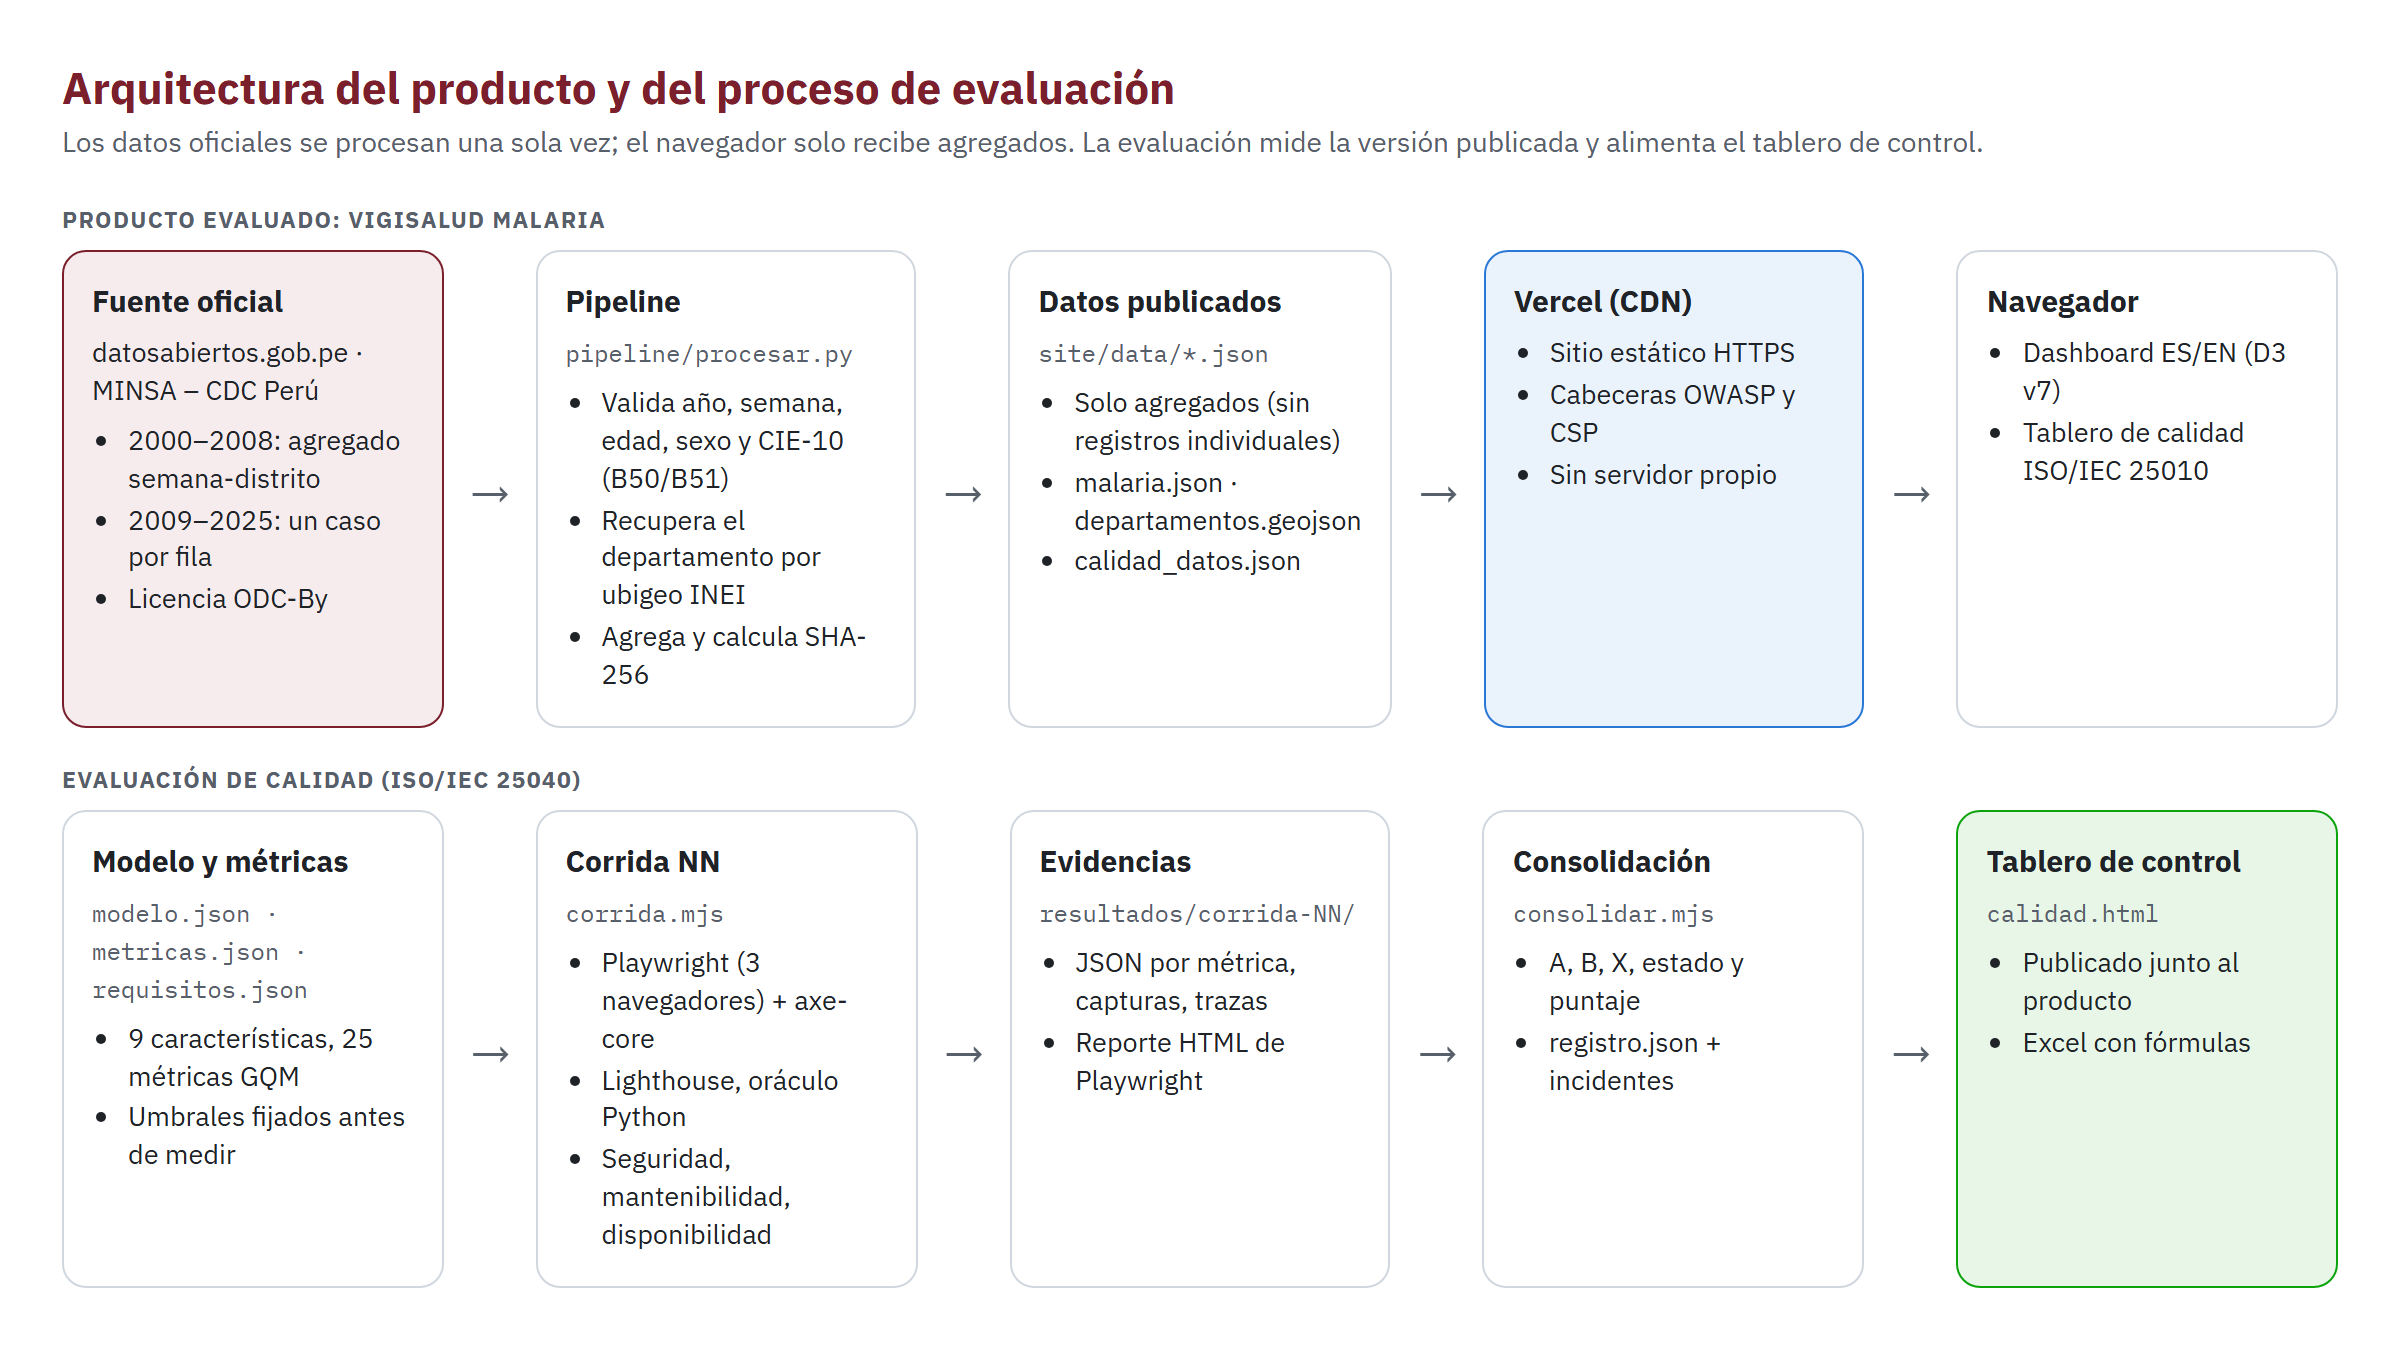
\includegraphics[width=0.92\textwidth]{es-diag-arquitectura.png}
\caption{Arquitectura del producto y del proceso de evaluación. El tablero de control se genera desde las evidencias de cada corrida.}
\label{fig:arq}
\end{figure*}

\begin{figure}[t]
\centering
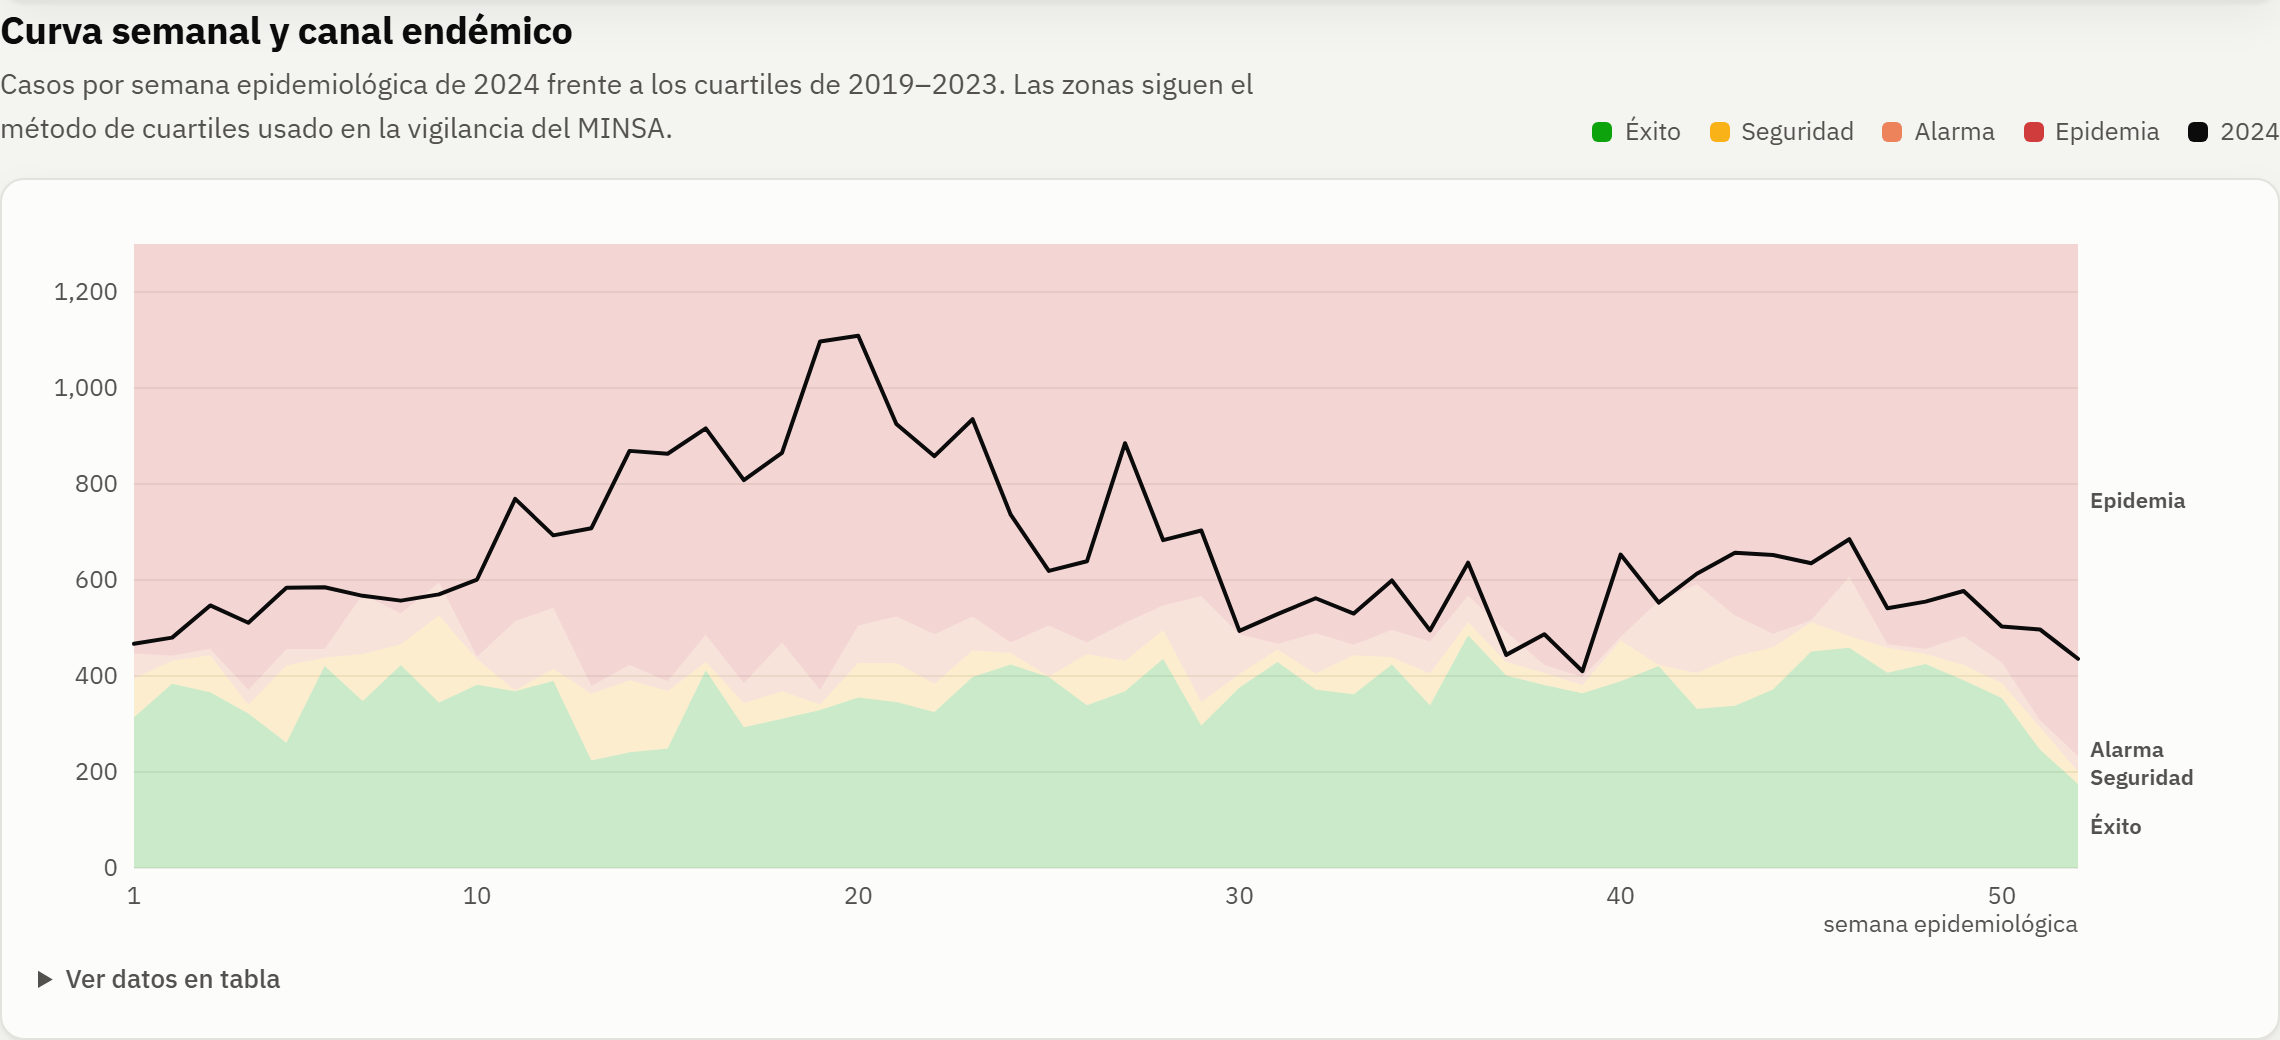
\includegraphics[width=\columnwidth]{es-canal.png}
\caption{Canal endémico semanal del dashboard (zonas de éxito, seguridad, alarma y epidemia).}
\label{fig:canal}
\end{figure}

\section{Modelo de calidad adoptado}
La prioridad de cada característica refleja el impacto de un defecto en un sistema que informa cifras para decisiones sanitarias (Tabla~\ref{tab:car}). Idoneidad funcional, capacidad de interacción, fiabilidad, seguridad y seguridad operacional son de prioridad alta. Las 14 subcaracterísticas excluidas se declaran \emph{no aplicables} cuando el producto carece de la propiedad (no repudio, autenticidad o instalabilidad en un sitio público de solo lectura) o \emph{no evaluadas} cuando requieren pruebas con usuarios (aprendizabilidad, reconocibilidad de la adecuación).

\begin{table}[t]
\caption{Características adoptadas, prioridad y métricas}
\label{tab:car}
\centering\footnotesize
\begin{tabular}{@{}L{2.6cm}lcL{2.6cm}@{}}
\toprule
Característica & Prior. & Subc. & Métricas \\
\midrule
Idoneidad funcional & Alta & 3/3 & IF-01 IF-02 IF-03 \\
Eficiencia de desempeño & Media & 2/3 & ED-01 ED-02 ED-03 \\
Compatibilidad & Baja & 1/2 & CO-01 \\
Capacidad de interacción & Alta & 4/6 & CI-01 CI-02 CI-03 CI-04 \\
Fiabilidad & Alta & 4/4 & FI-01 FI-02 FI-03 FI-04 \\
Seguridad & Alta & 3/6 & SE-01 SE-02 SE-03 \\
Mantenibilidad & Media & 3/5 & MA-01 MA-02 MA-03 \\
Flexibilidad & Media & 1/4 & FL-01 \\
Seguridad operacional & Alta & 3/5 & SO-01 SO-02 SO-03 \\
\bottomrule
\end{tabular}
\end{table}

\section{Métricas}
Cada métrica tiene objetivo, pregunta, $A$, $B$, fórmula, unidad, sentido, umbral, requisito, procedimiento, herramienta y responsable. Las métricas de proporción usan $X=A/B\times100$ como puntaje; las de valor en las que menor es mejor (LCP, tiempo de respuesta, peso, densidad de problemas) se normalizan como $\min(100,\,100\cdot u/X)$. Los umbrales se fijaron antes de la corrida~01. La corrección funcional (IF-02) no se verifica con el código que produce las cifras: un oráculo independiente recalcula desde los CSV los valores esperados de ocho escenarios y la prueba compara cada cifra visible (84 comparaciones).

\section{Proceso y formato de recopilación}
El proceso adapta las cinco actividades de ISO/IEC~25040 con responsables y un ciclo de mejora (Fig.~\ref{fig:proc}). Una corrida se lanza con un comando que registra las condiciones (fecha, versión, URL, entorno, navegadores y hashes de los datos), ejecuta Playwright en Chromium, Firefox y WebKit con axe-core (WCAG~2.2 A/AA \cite{wcag}), Lighthouse en perfil móvil, controles de cabeceras OWASP \cite{owasp} e integridad, ESLint y Radon (complejidad ciclomática \cite{mccabe}), y 20 sondeos HTTP de disponibilidad. Cada medición genera una ficha de siete bloques: identificación, trazabilidad, condiciones, medición, evaluación, evidencia y seguimiento.

\begin{figure}[t]
\centering
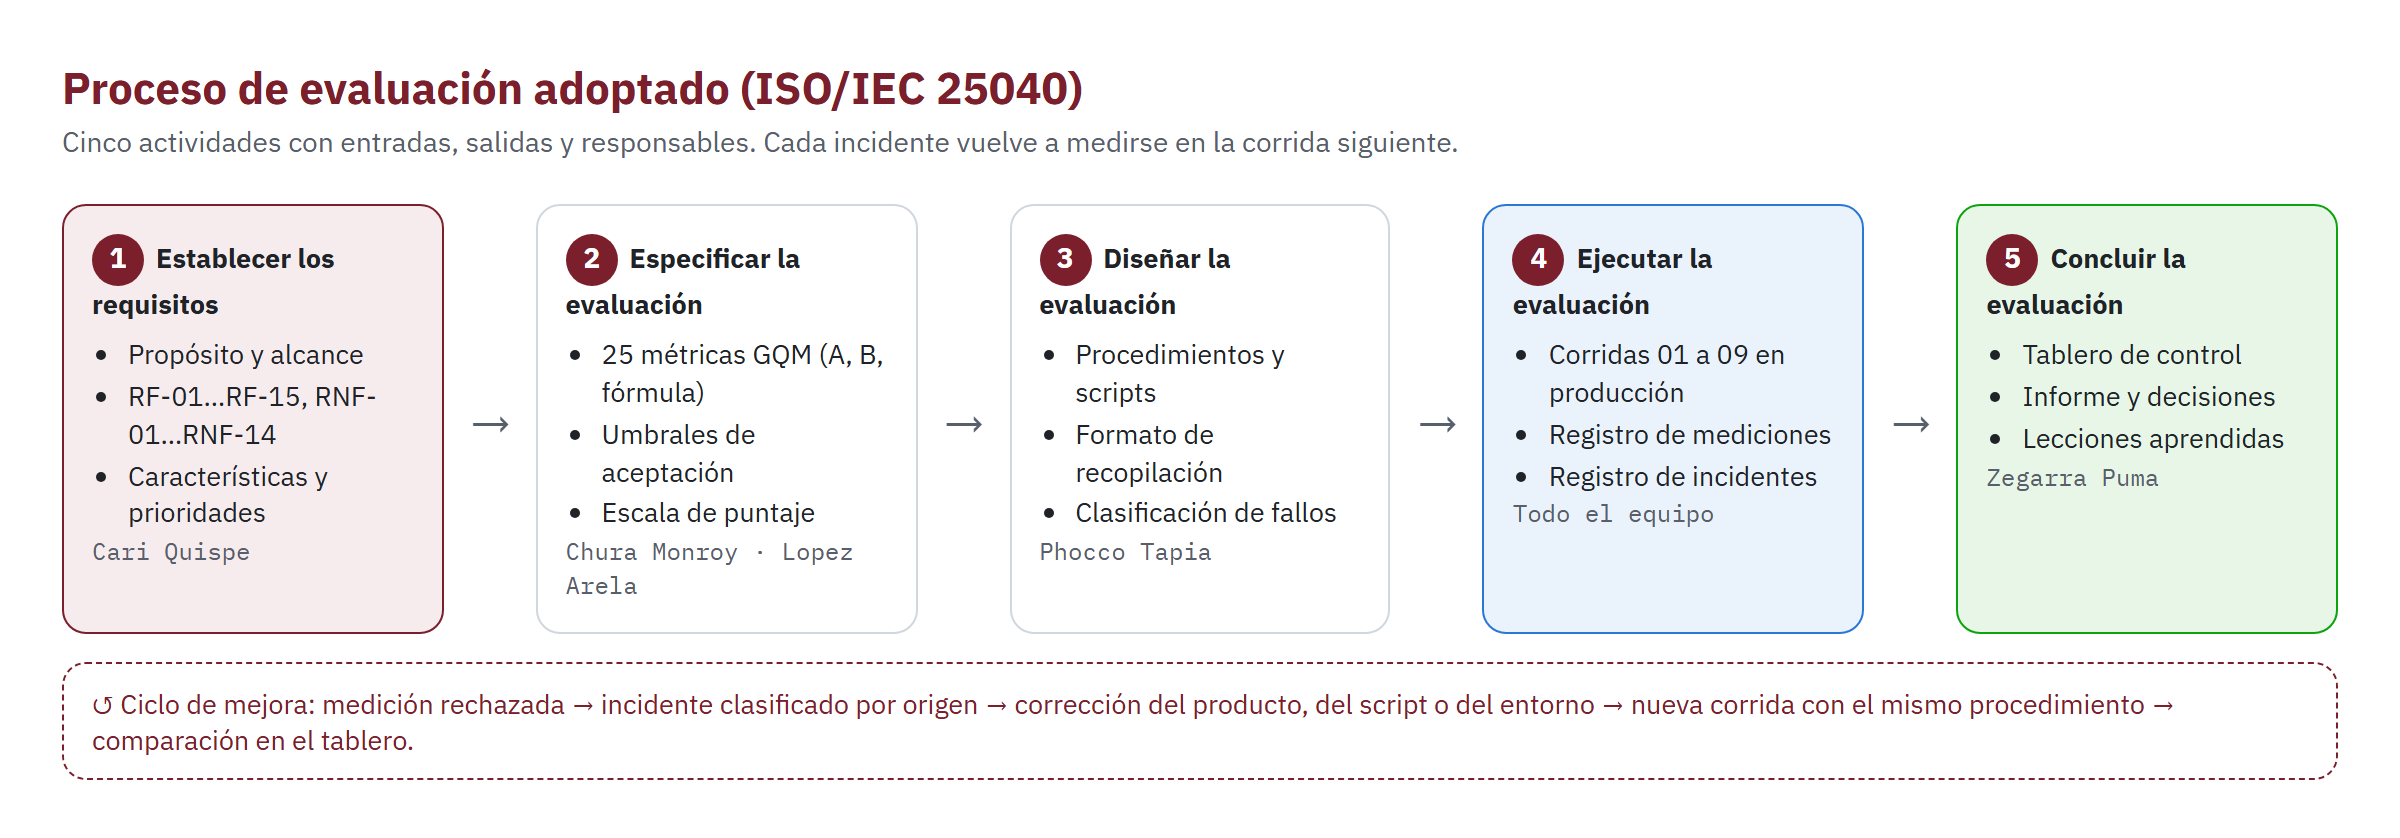
\includegraphics[width=\columnwidth]{es-diag-proceso.png}
\caption{Proceso de evaluación adoptado (ISO/IEC 25040) con ciclo de mejora.}
\label{fig:proc}
\end{figure}

Antes de corregir, cada fallo se reproduce y se clasifica por origen (Fig.~\ref{fig:origen}): \emph{producto} si el defecto aparece en la versión publicada, \emph{script} si el producto es correcto y el error está en la prueba o en el registro de la medición, e \emph{infraestructura} si depende del entorno de ejecución.

\begin{figure}[t]
\centering
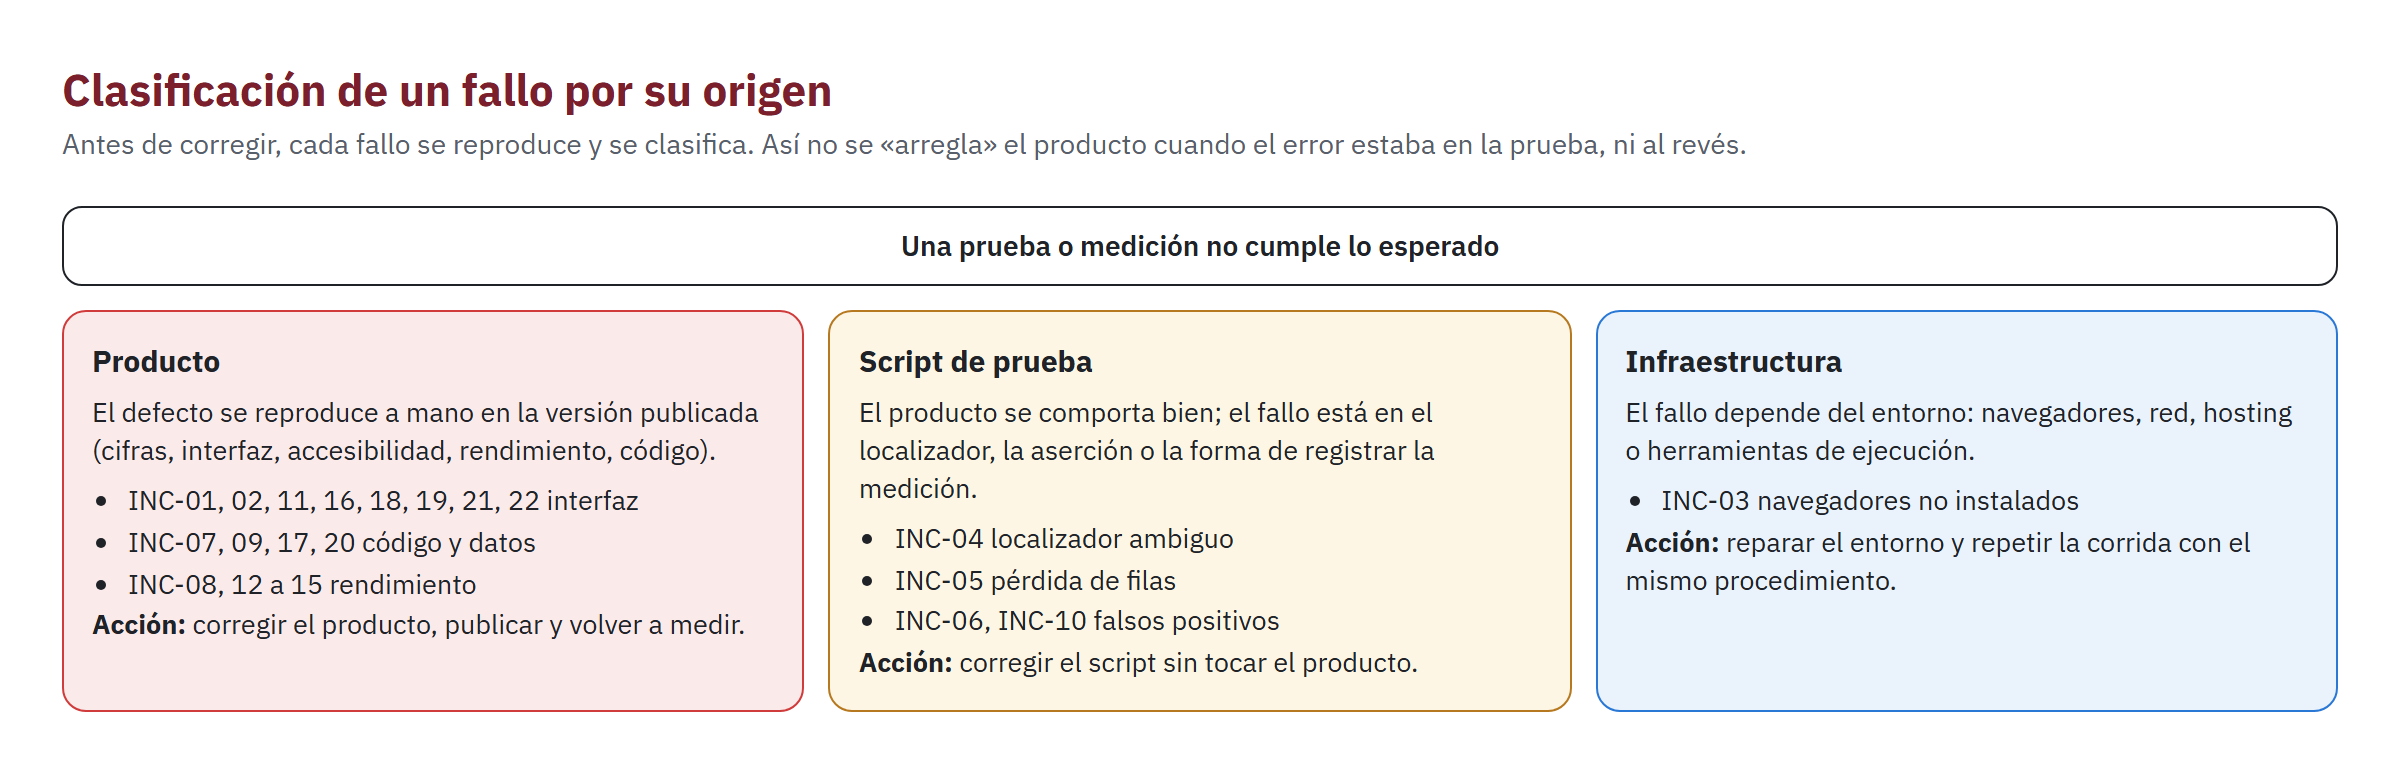
\includegraphics[width=\columnwidth]{es-diag-origen.png}
\caption{Regla de clasificación de fallos por origen.}
\label{fig:origen}
\end{figure}

\section{Resultados}
La Tabla~\ref{tab:res} muestra las 25 métricas en las 9 corridas. Las métricas aprobadas fueron 18, 24, 24, 24, 25, 25, 25, 25, 25 de 25, y las pruebas automatizadas aprobadas, 40/51, 51/51, 51/51, 51/51, 51/51, 51/51, 51/51, 51/51, 51/51. IF-02 no encontró ninguna diferencia con el oráculo en ninguna corrida.

\begin{table*}[t]
\caption{Resultado $X$ por corrida ($^{\ast}$ no cumple el umbral)}
\label{tab:res}
\centering\scriptsize
\setlength{\tabcolsep}{4pt}
\begin{tabular}{@{}lL{4.8cm}lccccccccc@{}}
\toprule
ID & Métrica & Umbral & C01 & C02 & C03 & C04 & C05 & C06 & C07 & C08 & C09 \\
\midrule
IF-01 & Cobertura de requisitos funcionales & $\geq$95\,\% & 93{,}3$^{\ast}$ & 100{,}0 & 100{,}0 & 100{,}0 & 100{,}0 & 100{,}0 & 100{,}0 & 100{,}0 & 100{,}0 \\
IF-02 & Exactitud frente al oráculo oficial & $\geq$100\,\% & 100{,}0 & 100{,}0 & 100{,}0 & 100{,}0 & 100{,}0 & 100{,}0 & 100{,}0 & 100{,}0 & 100{,}0 \\
IF-03 & Cobertura de las dimensiones de vigilancia & $\geq$90\,\% & 100{,}0 & 100{,}0 & 100{,}0 & 100{,}0 & 100{,}0 & 100{,}0 & 100{,}0 & 100{,}0 & 100{,}0 \\
ED-01 & Largest Contentful Paint (móvil) & $\leq$2{,}5\,s & 3{,}29$^{\ast}$ & 2{,}48 & 2{,}56$^{\ast}$ & 2{,}55$^{\ast}$ & 0{,}98 & 0{,}98 & 0{,}98 & 0{,}98 & 0{,}98 \\
ED-02 & Tiempo de respuesta a filtros & $\leq$200\,ms & 42{,}80 & 42{,}40 & 38{,}50 & 38{,}50 & 36{,}90 & 36{,}60 & 37{,}10 & 38{,}80 & 39{,}20 \\
ED-03 & Peso transferido en la carga inicial & $\leq$1~000\,KB & 276{,}12 & 333{,}27 & 333{,}29 & 333{,}71 & 334{,}12 & 334{,}08 & 334{,}62 & 334{,}79 & 334{,}80 \\
CO-01 & Exportaciones válidas y consistentes & $\geq$100\,\% & 100{,}0 & 100{,}0 & 100{,}0 & 100{,}0 & 100{,}0 & 100{,}0 & 100{,}0 & 100{,}0 & 100{,}0 \\
CI-01 & Controles operables con teclado & $\geq$95\,\% & 100{,}0 & 100{,}0 & 100{,}0 & 100{,}0 & 100{,}0 & 100{,}0 & 100{,}0 & 100{,}0 & 100{,}0 \\
CI-02 & Entradas inválidas controladas & $\geq$100\,\% & 100{,}0 & 100{,}0 & 100{,}0 & 100{,}0 & 100{,}0 & 100{,}0 & 100{,}0 & 100{,}0 & 100{,}0 \\
CI-03 & Violaciones WCAG graves & $\geq$100\,\% & 0{,}0$^{\ast}$ & 100{,}0 & 100{,}0 & 100{,}0 & 100{,}0 & 100{,}0 & 100{,}0 & 100{,}0 & 100{,}0 \\
CI-04 & Gráficos con alternativa textual & $\geq$100\,\% & 100{,}0 & 100{,}0 & 100{,}0 & 100{,}0 & 100{,}0 & 100{,}0 & 100{,}0 & 100{,}0 & 100{,}0 \\
FI-01 & Ejecuciones sin errores de JavaScript & $\geq$100\,\% & 33{,}3$^{\ast}$ & 100{,}0 & 100{,}0 & 100{,}0 & 100{,}0 & 100{,}0 & 100{,}0 & 100{,}0 & 100{,}0 \\
FI-02 & Disponibilidad medida & $\geq$99\,\% & 100{,}0 & 100{,}0 & 100{,}0 & 100{,}0 & 100{,}0 & 100{,}0 & 100{,}0 & 100{,}0 & 100{,}0 \\
FI-03 & Fallos de datos controlados & $\geq$100\,\% & 100{,}0 & 100{,}0 & 100{,}0 & 100{,}0 & 100{,}0 & 100{,}0 & 100{,}0 & 100{,}0 & 100{,}0 \\
FI-04 & Recuperación tras el fallo & $\geq$100\,\% & 100{,}0 & 100{,}0 & 100{,}0 & 100{,}0 & 100{,}0 & 100{,}0 & 100{,}0 & 100{,}0 & 100{,}0 \\
SE-01 & Ausencia de microdatos publicados & $\geq$100\,\% & 66{,}7$^{\ast}$ & 66{,}7$^{\ast}$ & 100{,}0 & 100{,}0 & 100{,}0 & 100{,}0 & 100{,}0 & 100{,}0 & 100{,}0 \\
SE-02 & Integridad de los datos de origen & $\geq$100\,\% & 100{,}0 & 100{,}0 & 100{,}0 & 100{,}0 & 100{,}0 & 100{,}0 & 100{,}0 & 100{,}0 & 100{,}0 \\
SE-03 & Cabeceras de seguridad OWASP & $\geq$85\,\% & 100{,}0 & 100{,}0 & 100{,}0 & 100{,}0 & 100{,}0 & 100{,}0 & 100{,}0 & 100{,}0 & 100{,}0 \\
MA-01 & Funciones con complejidad aceptable & $\geq$90\,\% & 98{,}2 & 99{,}0 & 99{,}0 & 99{,}0 & 99{,}0 & 99{,}0 & 99{,}0 & 99{,}0 & 99{,}0 \\
MA-02 & Densidad de problemas de análisis estático & $\leq$2\,problemas/KLOC & 3{,}01$^{\ast}$ & 0{,}00 & 0{,}00 & 0{,}00 & 0{,}00 & 0{,}00 & 0{,}00 & 0{,}00 & 0{,}00 \\
MA-03 & Requisitos con prueba automatizada & $\geq$90\,\% & 100{,}0 & 100{,}0 & 100{,}0 & 100{,}0 & 100{,}0 & 100{,}0 & 100{,}0 & 100{,}0 & 100{,}0 \\
FL-01 & Combinaciones navegador $\times$ pantalla correctas & $\geq$100\,\% & 33{,}3$^{\ast}$ & 100{,}0 & 100{,}0 & 100{,}0 & 100{,}0 & 100{,}0 & 100{,}0 & 100{,}0 & 100{,}0 \\
SO-01 & Vistas con aviso de datos provisionales & $\geq$100\,\% & 100{,}0 & 100{,}0 & 100{,}0 & 100{,}0 & 100{,}0 & 100{,}0 & 100{,}0 & 100{,}0 & 100{,}0 \\
SO-02 & Sin cifras parciales ante fallos & $\geq$100\,\% & 100{,}0 & 100{,}0 & 100{,}0 & 100{,}0 & 100{,}0 & 100{,}0 & 100{,}0 & 100{,}0 & 100{,}0 \\
SO-03 & Limitaciones de la fuente señaladas & $\geq$100\,\% & 100{,}0 & 100{,}0 & 100{,}0 & 100{,}0 & 100{,}0 & 100{,}0 & 100{,}0 & 100{,}0 & 100{,}0 \\
\bottomrule
\end{tabular}
\end{table*}

En la corrida~01, los rechazos tuvieron orígenes distintos (Tabla~\ref{tab:inc}). Dos violaciones \emph{serious} de axe-core afectaban al producto. El LCP móvil fue de 3{,}29\,s por una hoja de estilos de fuentes de terceros que bloqueaba el render; tras servir las fuentes desde el mismo origen y precargar los datos bajó a 2{,}48\,s. Firefox y WebKit no estaban instalados, lo que dejaba sin medir seis de las nueve combinaciones de adaptabilidad: por eso FL-01 usa como denominador los casos planificados y no los ejecutados. La corrida~02 mostró dos regresiones introducidas por correcciones (el logotipo sin nombre accesible en móvil y un CLS de 0,11 por el cambio de fuente) y un falso positivo residual del control de confidencialidad. La corrida~03 mostró que el CLS persistía: la atribución de Lighthouse apuntaba a las fuentes, pero al medir los desplazamientos con \texttt{PerformanceObserver} en el mismo viewport apareció la causa real, una cuadrícula móvil que estiraba la barra superior mientras el contenido no estaba cargado. Era un defecto latente que la mejora del FCP dejó a la vista. Además, el elemento LCP dependía de los datos para pintarse (2{,}56\,s). En la corrida~04 el aviso ya era estático, pero el LCP simulado siguió en 2{,}55\,s: el modelo Lantern de Lighthouse cuenta todas las peticiones iniciadas antes del primer pintado, y las precargas de datos y fuentes que habían ayudado en la corrida~02 ya solo competían por el ancho de banda. Se pidieron los datos y D3 después del primer pintado, y en la corrida~09 el LCP fue de 0{,}98\,s. Por último, la revisión manual de las capturas de la corrida~05 encontró una leyenda con los nombres de especie recortados desde la v1.0 (INC-16); CI-04 no lo detectaba porque comprueba que la leyenda exista, no que sea legible. Las revisiones siguientes encontraron nombres con la Ñ dañada en los archivos oficiales, etiquetas superpuestas y textos en español en la interfaz inglesa. Este último se resolvió con un barrido automático del texto visible, que a su vez hubo que ampliar a los valores enumerados del modelo cuando la inspección visual encontró un resto que el barrido no detectaba (INC-22). La Fig.~\ref{fig:evo} muestra la evolución en el tablero.

\begin{table*}[t]
\caption{Incidentes registrados y su origen}
\label{tab:inc}
\centering\scriptsize
\setlength{\tabcolsep}{4pt}
\begin{tabular}{@{}lccL{1.9cm}L{12.4cm}@{}}
\toprule
ID & C & Métrica & Origen & Causa \\
\midrule
INC-01 & 01 & CI-03 & producto & Etiqueta accesible fija que sobrescribe el texto visible (WCAG 2.5.3 Etiqueta en el nombre). \\
INC-02 & 01 & CI-03 & producto & Los .tablewrap tienen overflow:auto sin tabindex ni rol (WCAG 2.1.1 Teclado). \\
INC-03 & 01 & FL-01 & infraestructura & Tras actualizar @playwright/test a 1.64.1 solo estaba instalado el binario de Chromium. \\
INC-04 & 01 & IF-01 & script & Localizador ambiguo por nombre accesible parcial. \\
INC-05 & 01 & CI-03 & script & El registro de mediciones escribía el archivo solo en afterAll. \\
INC-06 & 01 & SE-01 & script & El script comparaba solo nombres de claves, sin mirar el tipo de valor. \\
INC-07 & 01 & MA-02 & producto & Variables de captura declaradas y no utilizadas. \\
INC-08 & 01 & ED-01 & producto & CSS de fuentes de terceros bloqueante y descarga de datos que empezaba recién al ejecutarse app.js. \\
INC-09 & 01 & MA-01 & producto & Cálculo y presentación de los cinco indicadores en una sola función. \\
INC-10 & 02 & SE-01 & script & La regla de INC-06 miraba el tipo del valor pero no si el campo pertenecía a un registro. \\
INC-11 & 02 & CI-03 & producto & El texto del logotipo se ocultaba con display:none en pantallas pequeñas, lo que también lo retira del árbol de accesibilidad. \\
INC-12 & 02 & ED-01 & producto & Con swap, el texto se pinta primero con la fuente del sistema y se recoloca al llegar IBM Plex. \\
INC-13 & 03 & ED-01 & producto & Filas auto de la cuadrícula móvil que reparten el espacio libre mientras el contenido aún no se ha cargado. \\
INC-14 & 03 & ED-01 & producto & El elemento más grande del viewport dependía de los datos para pintarse. \\
INC-15 & 04 & ED-01 & producto & Recursos que no participan en el primer pintado se pedían antes que él. \\
INC-16 & 05 & CI-04 & producto & Conflicto de selector: la misma etiqueta <i> servía de muestra de color y de cursiva. \\
INC-17 & 06 & IF-03 & producto & Fallo de codificación en la fuente, no tratado por el pipeline. \\
INC-18 & 06 & CI-04 & producto & Cada etiqueta se ubicaba en el centro de su banda sin controlar la distancia con las demás. \\
INC-19 & 06 & IF-03 & producto & Cuadrícula de dos columnas automáticas para etiquetas de longitud muy distinta. \\
INC-20 & 06 & SE-02 & producto & Se confundía la fecha de procesamiento con la de descarga. \\
INC-21 & 07 & IF-01 & producto & Los textos que provienen de los datos de evaluación (modelo.json, requisitos.json) y de los motivos de validación no tenían versión en inglés. \\
INC-22 & 08 & IF-01 & producto & Valor enumerado del modelo mostrado sin traducir; barrido incompleto. \\
\bottomrule
\end{tabular}
\end{table*}

\begin{figure}[t]
\centering
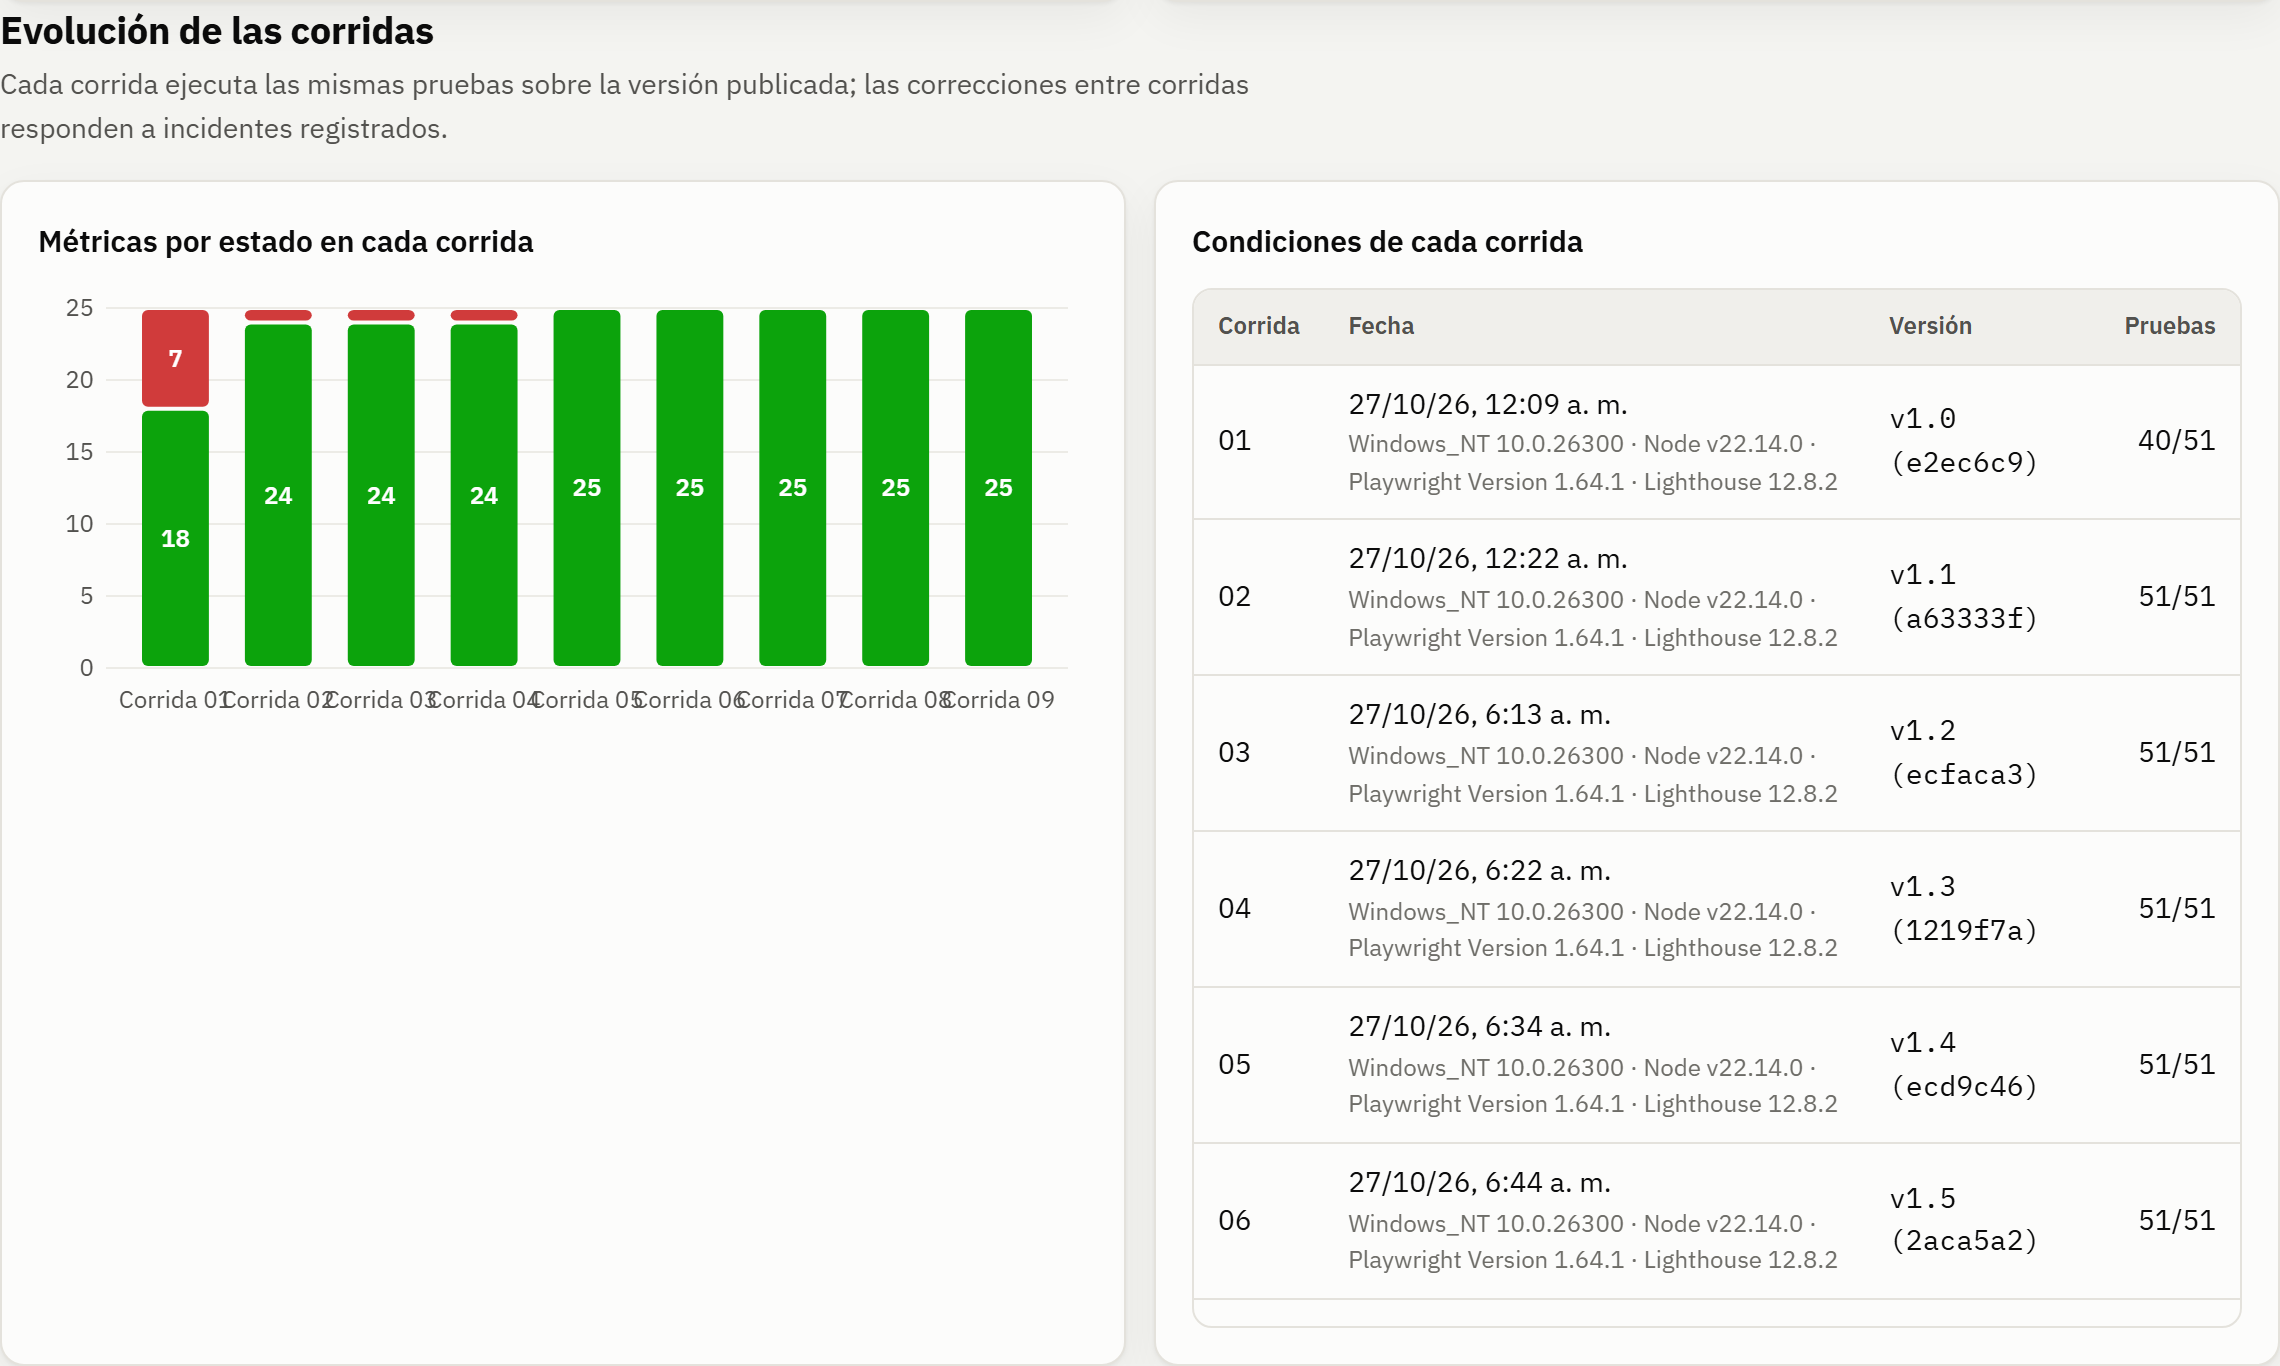
\includegraphics[width=\columnwidth]{es-calidad-evolucion.png}
\caption{Tablero de control: evolución de las métricas aprobadas por corrida.}
\label{fig:evo}
\end{figure}

\section{Discusión}
De 22 incidentes, 5 no eran defectos del producto. Sin la clasificación por origen, el equipo habría modificado el producto por fallos de sus propias pruebas o de su entorno, y habría reportado una calidad menor que la real. A la vez, dos correcciones del producto introdujeron regresiones que solo aparecieron al repetir la medición completa, lo que justifica exigir una corrida nueva tras cada cambio. Un incidente tampoco debe cerrarse con la explicación de la herramienta, sino cuando la medición siguiente lo confirma: INC-12 parecía resuelto y no lo estaba. Un punto ciego concreto fue que axe-core se ejecutaba solo en escritorio y la regresión del logotipo apareció en móvil; se recomienda incluir una vista móvil en CI-03. Otro fue INC-16: una métrica que verifica la presencia de un elemento no garantiza su legibilidad, por lo que la revisión visual de las evidencias debe mantenerse como paso del proceso.

\emph{Amenazas a la validez.} El rendimiento se midió con el perfil móvil simulado de Lighthouse desde una sola ubicación; la disponibilidad, con sondeos durante cada corrida y no con monitoreo continuo. Las subcaracterísticas que requieren usuarios no se evaluaron. El equipo evaluó un producto propio; para mitigar el sesgo, los umbrales se fijaron antes de medir, el oráculo es independiente del código evaluado y todas las evidencias son públicas.

\section{Conclusiones}
Se aplicó ISO/IEC~25010:2023 de extremo a extremo a un dashboard real de vigilancia de malaria: modelo con prioridades y exclusiones justificadas, 25 métricas GQM automatizadas, un proceso basado en ISO/IEC~25040 con un formato de recopilación trazable y un tablero de control público. Las métricas aprobadas pasaron de 18 a 25 de 25 en 9 corridas. Como trabajo futuro se propone ejecutar la corrida en integración continua con bloqueo de despliegue y completar la evaluación con pruebas de usuario.

\begin{thebibliography}{10}
\bibitem{iso25010} ISO/IEC 25010:2023, \emph{Systems and software engineering --- SQuaRE --- Product quality model}, ISO, Ginebra, 2023.
\bibitem{iso25040} ISO/IEC 25040:2024, \emph{Systems and software engineering --- SQuaRE --- Quality evaluation framework}, ISO, Ginebra, 2024.
\bibitem{iso25023} ISO/IEC 25023:2016, \emph{Systems and software engineering --- SQuaRE --- Measurement of system and software product quality}, ISO, Ginebra, 2016.
\bibitem{basili} V.~R. Basili, G.~Caldiera y H.~D. Rombach, ``The goal question metric approach,'' en \emph{Encyclopedia of Software Engineering}, Wiley, 1994.
\bibitem{calabrese} J.~Calabrese, R.~Muñoz, A.~Pasini, S.~Esponda, M.~Boracchia y P.~Pesado, ``Assistant for the evaluation of software product quality characteristics proposed by ISO/IEC 25010 based on GQM-defined metrics,'' en \emph{Computer Science -- CACIC 2017}, CCIS, vol.~790, Springer, 2018, pp.~164--175.
\bibitem{minsa} MINSA -- CDC Perú, ``Vigilancia epidemiológica de malaria,'' Plataforma Nacional de Datos Abiertos, descargado el 26/10/2026. [En línea]. Disponible: \url{https://www.datosabiertos.gob.pe/dataset/vigilancia-epidemiol\%C3\%B3gica-de-malaria}
\bibitem{bortman} M.~Bortman, ``Elaboración de corredores o canales endémicos mediante planillas de cálculo,'' \emph{Rev. Panam. Salud Pública}, vol.~5, n.º~1, pp.~1--8, 1999.
\bibitem{wcag} W3C, \emph{Web Content Accessibility Guidelines (WCAG) 2.2}, 2023.
\bibitem{owasp} OWASP Foundation, \emph{OWASP Secure Headers Project}. [En línea]. Disponible: \url{https://owasp.org/www-project-secure-headers/}
\bibitem{mccabe} T.~J. McCabe, ``A complexity measure,'' \emph{IEEE Trans. Softw. Eng.}, vol.~SE-2, n.º~4, pp.~308--320, 1976.
\end{thebibliography}

\end{document}
